\documentclass[runningheads]{llncs}

% PACKAGES
\usepackage[T1]{fontenc}
\usepackage{lmodern}
\usepackage{textcomp}
\usepackage{graphicx}
\usepackage{booktabs}
\usepackage[indentfirst=false,font={itshape},begintext=``,endtext='']{quoting}
\usepackage{subcaption}
\usepackage[hyphens,spaces,obeyspaces]{url}
\usepackage{hyperref}
\usepackage[backend=biber,style=acmnumeric,doi=true,url=true]{biblatex}
\addbibresource{helios_prototype.bib}
\usepackage[most]{tcolorbox}
\usepackage{tabularx,ragged2e}
\newtcolorbox{summarybox}{
    enhanced,
    breakable,
    sharp corners,
    boxrule=0.3pt,
    colback=white,
    colframe=black!40,
    coltitle=black,
    fonttitle=\bfseries,
    toptitle=2mm,
    bottomtitle=2mm,
    colbacktitle=white,
}
\usepackage{cleveref}
\usepackage{longtable}
\usepackage[titletoc,title,page, header]{appendix} %

\DeclareFieldFormat{doi}{\textsc{doi}: \texttt{#1}}
\DeclareFieldFormat{isbn}{\textsc{isbn}: \texttt{#1}}
\usepackage{dirtree}
\renewcommand*\DTstyle{\ttfamily}
\usepackage{listings}
\usepackage{xcolor}
\definecolor{codegray}{gray}{0.9}
\definecolor{commentgreen}{rgb}{0,0.6,0}
\definecolor{keywordblue}{rgb}{0.2,0.2,0.8}

\lstdefinestyle{c++style}{
    backgroundcolor=\color{white},
    commentstyle=\color{commentgreen}\itshape,
    keywordstyle=\color{keywordblue}\bfseries,
    numberstyle=\tiny\color{gray},
    stringstyle=\color{red},
    basicstyle=\ttfamily\small,
    breaklines=true,
    captionpos=b,
    keepspaces=true,
    numbers=left,
    numbersep=5pt,
    showspaces=false,
    showstringspaces=false,
    showtabs=false,
    tabsize=2,
    language=C++
}

% linksbündig und automatischer Umbruch
\newcolumntype{Y}{>{\RaggedRight\arraybackslash}X}

\usepackage[english, ngerman]{babel}
\usepackage{bibgerm}

\begin{document}

% title and authors
    \title{helios: Konzeption und prototypische Umsetzung eines C++ Game Frameworks}
    \titlerunning{helios: Konzeption und prototypische Umsetzung}
    \author{
        Thorsten Suckow-Homberg
    }

% First names are abbreviated in the running head.
% If there are more than two authors, 'et al.' is used.
    \authorrunning{T. Suckow-Homberg}
    \institute{Trier University of Applied Sciences \\ \email{thorsten@suckow-homberg.de} \\
    01.11.2025}

% typeset the header of the contribution
    \maketitle

% sub names
% eg
%\newcommand{\saud}[1]{\textit{Audio (AUD)}}


    \begin{abstract}
    Wir stellen \textit{helios} vor, einen in C++23 entworfenen Prototypen einer Game-Engine zur Entwicklung eines Geometry Wars Klons. Wir beschreiben den grundlegenden Aufbau des Frameworks vor und beschreiben Sinn und Zweck der einzelen Module. Wir gehen auf Architektur- und Designentscheidungen ein und beschreiben Schwierigkeiten bei dem Entwicklungsprozess. Wir schließen mit einem Ausblick ab, an welchen Stellen wir im Verlauf der weiteren Entwicklung die größten Änderungen erwarten.
\end{abstract}


\section{Einleitung}

Wir programmieren einen \textit{Geometry Wars}\footnote{siehe~\cite[]{WikipediaGeometryWars}} Klon in C++.
Bei der Umsetzung orientieren wir uns teilweise an einer in der Industrie weit verbreiteten, von \textit{Gregory} in~\cite[]{Gre19} beschriebenen \textit{Game Engine Architektur}, reduzieren jedoch bewusst die Anzahl der Abstraktionsschichten und verzichten auf Systeme wie Tooling, Sound oder Scripting (vgl.~\cite[\textbf{Figure 1.16}, 39]{Gre19}), so dass die \textit{Hard Architecture}~\cite[]{RM04} einem Framework entspricht, welches Schnittstellen für benötigte Hardware und andere Subsysteme bereitstellt, die dem eigentlichen Spiel als technischer Unterbau dienen.
Das Spiel selber wird - als \textit{Black Box}~\cite[]{RB88} - von diesen Schnittstellen Gebrauch machen.\\

\begin{figure}[!h]
    \centering
    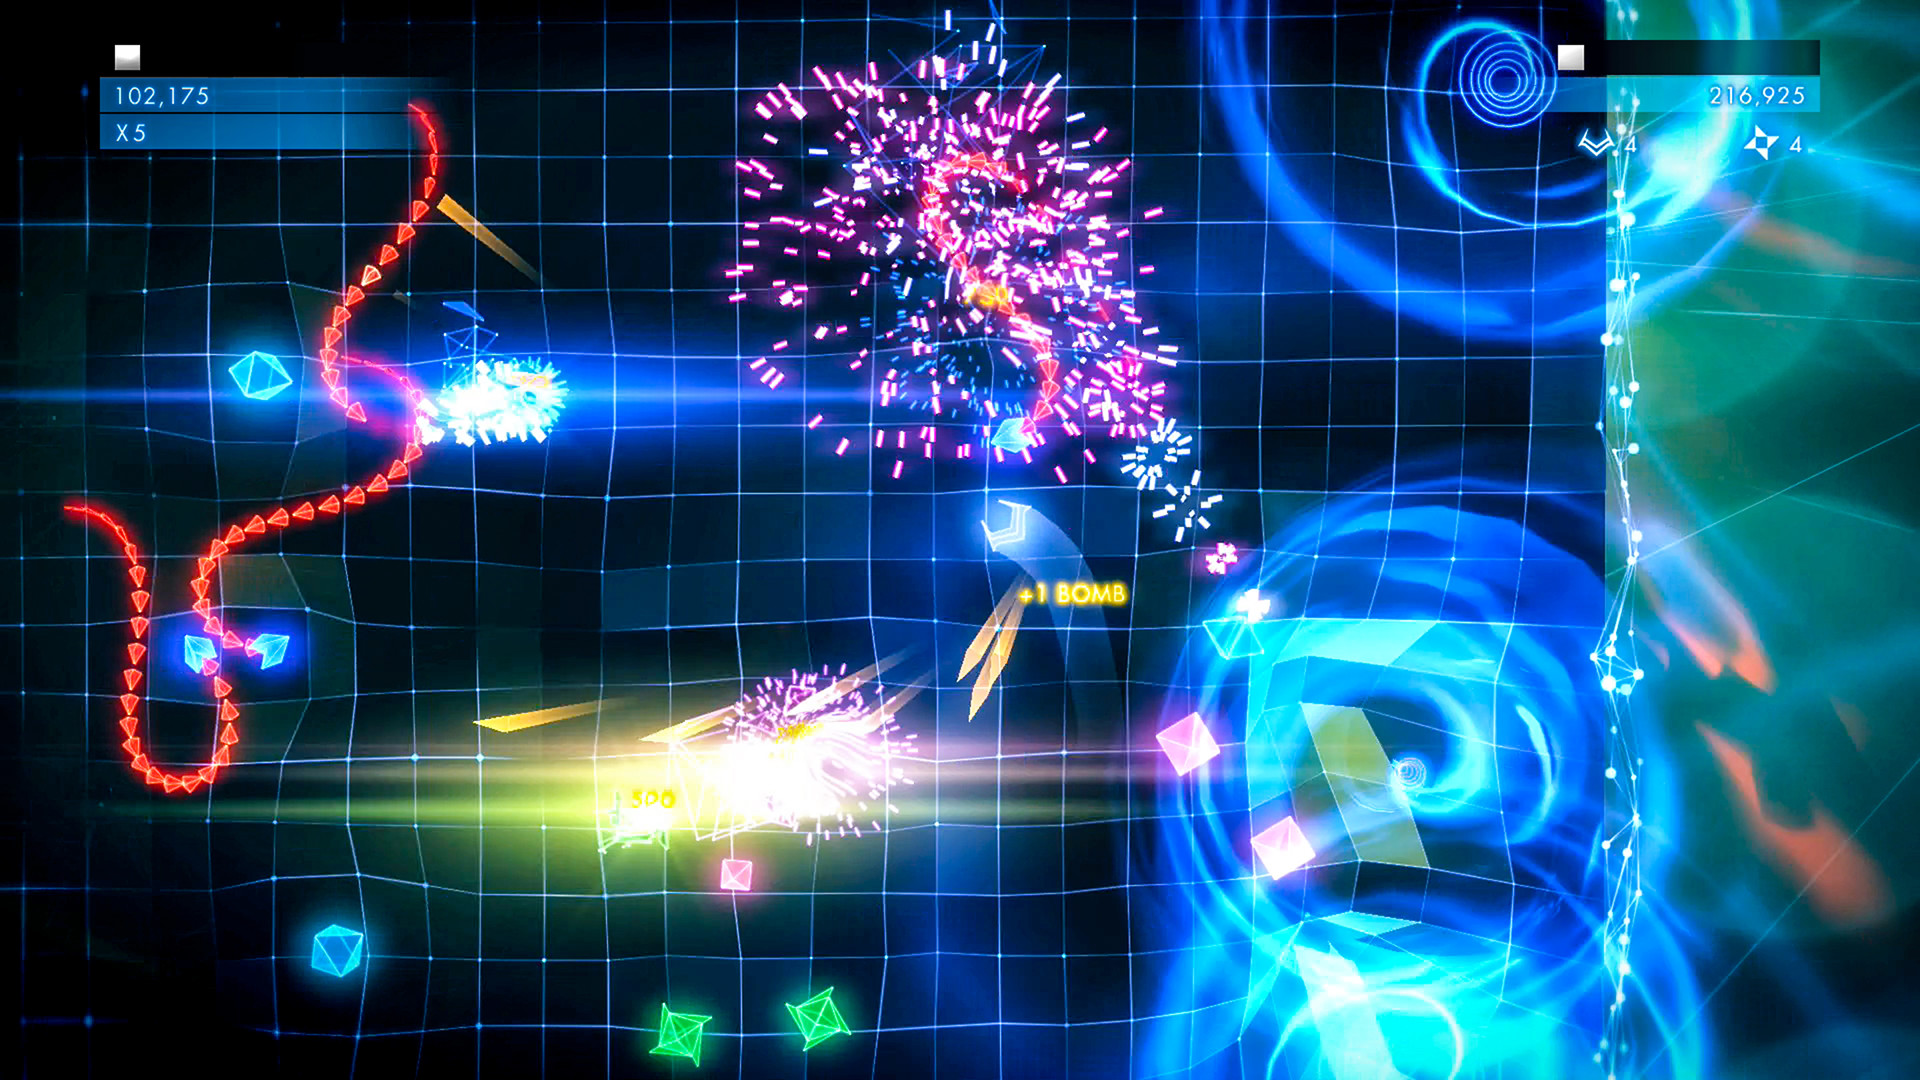
\includegraphics[width=1\columnwidth]{img/geometry_wars}
    \caption{Geometry Wars fand sich erstmals 2003 als Easter Egg in dem Spiel \textit{Project Gotham Racing} (Microsoft Game Studios). Aufgrund der großen Beliebtheit entstanden mehrere Nachfolger, zuletzt 2016 mit \textit{Geometry Wars 3: Dimensions Evolved} (Activision). (Quelle: Steam)}
    \label{fig:geometry_wars}
\end{figure}

In den nachfolgenden Abschnitten wird die Architektur von dem mit \textbf{helios}\footnote{
    Helios, der ``scharf vor allen mit strahlenden Augen umherblickt`` (\textit{Homers Ilias}, 14. Gesang), ist in der griechischen Mythologie der Sonnengott.
} getauften Framework vorgestellt.
Dabei berücksichtigen wir, dass es sich um einen in der Entwicklung befindlichen Prototypen handelt:
Die Software wird im Rahmen eines agilen \textit{Tracer Bullet Development}-Prozess~\cite[50 f.]{TH20} entwickelt.
Dadurch soll das Gesamtsystem verhältnis- und zweckmäßig angepasst werden können, woraus sich auch Anforderungen an die Architektur ableiten lassen.
In Abschnitt~\ref{sec:projektdaten} wird noch einmal gesondert auf die Anforderungen eingegangen. \\

\begin{figure}[!h]
    \centering
    
\includegraphics[width=0.5\columnwidth]{img/helios_logo}
    \caption{Das helios Projekt-Logo.}
    \label{fig:helios_logo}
\end{figure}


Wir betrachten auch Probleme und Schwierigkeiten, die bei der bisherigen Umsetzung aufgetaucht sind.
Diese ergeben sich u.a. durch den Umstand, dass das in vergleichsweise kurzer Zeit zu erstellende Softwareprodukt nicht nur anhand \textit{objektiver} Maße bewertet werden soll (etwa der Fehleranzahl, Software-Designentscheidungen, Kopplungsgrad der Objekte etc.), sondern auch anhand \textit{subjektiver} Maße~\cite[385]{Bal08}.\\
Zwar ist keine Klassifizierung des fertigen Produkts nach Nutzungsqualitätsmerkmalen wie bspw. ISO/IEC 9126 angedacht\footnote{bspw. ``Nutzungsqualität nach ISO/IEC 9126``,~\cite[466]{Bal08}; Studien und Untersuchungen u.a. bei~\cite[]{AZMK17},~\cite[]{Ber10}}.
Dennoch soll das Ergebnis nicht nur technisch ausgereift sein, sondern auch für den Anwender angenehm zu bedienen.
Dieses Nutzererlebnis wird im Weiteren formal eher unscharf, aber mit dem in der Spieleentwicklung etablierten Begriff des \textit{Game Feel}~\cite[]{Swi08} zusammengefasst: Einem möglichst \textit{angenehmen} und in jeglicher Hinsicht \textit{positiven Spielerlebnis}.


\section{Projektziele und -daten}\label{sec:projektdaten}

Das Ziel der Projektarbeit ist es, einen stabil laufenden Prototyp des Twin-Stick Shooters\footnote{
Zur Genreeinteilung siehe auch \cite[]{GameDeveloper}
} \textit{Geometry Wars} (siehe Abbildung~\ref{fig:geometry_wars}) unter Verwendung der Programmiersprache \textit{C++} (23) und der OpenGL-API\footnote{siehe~\cite[]{OpenGLHomepage}
}  zu erstellen.\\

\noindent
Als grundsätzlich fertigzustellende Kernfeatures wurden vereinbart (siehe Anhang~\ref{sec:projektvorschlag}):

\vspace{2mm}
\begin{itemize}
    \itemsep0.5em
    \item Spielbares Level (2D-Grid)
    \item Time-Attack Modus mit einer Dauer von 3 Minuten
    \item Highscore-System
    \item Controller-Steuerung
    \item Stabile Framerate von mindestens 60 FPS bei gleichzeitiger Darstellung von über hundert Gegnern und Objekten
    \item Drei Gegnertypen mit einfacher KI (``Spawn and Chase``)
    \item Aufwertung des Game Feels durch grafische Effekte
    \item Compilierbar und lauffähig unter Windows 11
\end{itemize}
\vspace{2mm}

Die aufgeführten Punkte lassen nur vage Anforderungen erkennen, aus denen sich keine konkreten Abnahmekriterien ableiten lassen.
Ein \textit{Requirements Engineering} ist folglich auch nicht Bestandteil der Projektarbeit: Als ein Maß dient neben den o.a. funktionalen Kriterien vor allem auch das Original-Spiel, an dem sich die Umsetzung orientiert.\\

Insbesondere betrachten wir den \textit{Lernprozess} als ein wesentliches Ziel dieser Arbeit.
Für dessen Bewertung werden keine formalen Metriken herangezogen.
Stattdessen sollen die gewonnenen Erfahrungen und Ergebnisse im Anschluss schriftlich festgehalten und das hier vorliegende Dokument kritisch reflektiert werden.\\

Vor diesem Hintergrund wird das Vorgehen als eine Form des dynamischen Requirements Engineering ``mit deutlich größeren Freiheitsgeraden``~\cite[60]{MRP21} betrachtet: Das erwähnte \textit{Tracer Bullet Development}, das vor allem eine Plattform zur Integration bereitstellt, entspricht dem von \textit{Pflug et al.} mit ``Living Lab`` bezeichneten Prototyp, der im Weiteren nach agilen Methoden entwickelt wird (\textit{ebd., S. 61})\footnote{
    \textit{Kasurinen et al.} gehen in~\cite[]{KMS14} der Frage nach, ob das im Ingenieursbereich angesiedelte Anforderungsmanagement bei der stark durch kreative Prozesse beeinflussten Spieleentwicklung einen Platz hat. Sie zeigen, dass befragte Entwickler einen Teil der Anforderungen an ihr Spiel ganz bewusst erst durch \textit{User Testing} ableiten. Entsprechend stellt \textit{Games User Research} einen wichtigen Zweig der Spieleindustrie dar, der Unternehmen dabei unterstützt, Spiele-Erfahrung zu verstehen und zu verbessern (vgl.~\cite[26]{Zam18})
}, und ein Einbringen eigener kreativer Ideen erlauben soll.\\

\subsection{Zeitplan}

Wir stellen den Zeitplan vor und die aus dem Projektvorschlag übernommenen Meilensteinen, deren zeitliche Gliederung der Umsetzung dient\footnote{Aus der sequentiellen Auflistung soll kein Rückschluss auf ein Wasserfall-Modell gezogen werden}:

\vspace{2mm}
\begin{itemize}
    \itemsep0.5em
    \item \textbf{milestone\_1}: 20.10.2025: Bereitstellung der Applikationsschicht inkl. Implementierung des Event
    Systems, Input Managers sowie Anbindung an das Low Level API-Sub-Systems
    \item \textbf{milestone\_2}: 17.11.2025: Bereitstellung der Rendering Engine. Erster Entwurf des Spielfeldes
    samt Darstellung des Spielerschiffs.
    \item \textbf{milestone\_3}: 22.12.2025: Umsetzung der Physik und Spielereingabe zur Steuerung des Schiffs,
    Feuermechaniken
    \item \textbf{milestone\_4}: 19.01.2026: Implementierung der wichtigsten Spielregeln- und Mechaniken. Spiel
    fähiger Prototyp.
    \item \textbf{milestone\_5}: 09.02.2026: Bereitstellung des umgesetzten Prototyps. Feinschliff.
    \item \textbf{milestone\_6}: 16.03.2026: Abgabe der Dokumentation und Vorstellung des Projekts.
\end{itemize}
\vspace{2mm}

\noindent
Mit der Vorgabe des umzusetzenden Spielkonzeptes entfällt für uns dessen Prototyping.
Wir folgen \textit{Rollings und Morris} bei der Einordnung der gegenwärtigen Entwicklungsphase, die von den Autoren als \textit{hard-architecture design}-Phase bezeichnet wird (vgl.~\cite[628]{RM04}).\\

Zum Zeitpunkt der Veröffentlichung dieses Dokumentes ist der erste Meilenstein abgeschlossen: helios bietet bereits ein einfaches Fenstermanagement, rudimentäre Eingabe-Verarbeitung, ein Logging-System sowie ein funktionierendes Rendering Layer samt Anbindung an die OpenGL-API.\\

Das Projekt ist \textit{MIT} lizenziert auf Github veröffentlicht, Source Code und Ticketsystem sind öffentlich einsehbar~\cite[]{heliosgithub}.


\clearpage
\begin{appendices}
    
\section{Projektvorschlag vom 22.09.2025}\label{sec:projektvorschlag}

\section*{Schwerpunkt Rendering: Geometry Wars Klon}

\subsection{Anforderungen}

In der Projektarbeit wird ein Klon zu dem Spiel Geometry Wars\footnote{
\url{https://en.wikipedia.org/wiki/Geometry_Wars}
} erstellt, ein Top-Down Twin-Stick Shooter.\\

\noindent
Insgesamt dauert ein Spieldurchlauf 3 Minuten, oder bis der Spieler alle Schiffe verloren hat. Ziel ist es, die immer größer werdenden Gegnerwellen zu überdauern und dabei möglichst viel Punkte zu sammeln.



\subsection{Spielfunktionen}
\begin{itemize}
    \itemsep0.5em
    \item \textbf{Einzelspieler}
    \begin{itemize}
        \item Es gibt einen Spielmodus, den \textbf{Time-Attack-Modus}: Das Spiel gilt als erfolgreich beendet, wenn der Spieler eine Zeit von 3 Minuten überdauert.
    \end{itemize}
\end{itemize}

\subsection{Architektur}

Die Spieleengine ist nach \textit{first principles} aufgebaut und besitzt im Groben drei architektonische Schichten (s. Abbildung~\ref{fig:architecture}), die selbstständig erarbeitet werden:

\begin{enumerate}
    \item Applikationsschicht, die die Initialisierung und Verwaltung eines Event-Systems, Input Managers, Audio Managers und des Fenster Systems übernimmt. Notwendige SDKs, die diese Funktionen bereitstellen\footnote{
        sofern die Zeit es erlaubt, bspw. Audio wie \textbf{fmod} (\url{https://www.fmod.com})
    } sowie Fenstermanagement und Input (bspw. \textbf{glfw}\footnote{\url{https://www.glfw.org/}}), werden als vendor code von dem Spiel genutzt und über eine API gekapselt, damit die Applikationsschicht agnostisch hinsichtlich der verwendeten Libs ist (Adapter bzw. Wrapper).
    \item Render Engine: Als Rendering Backend wird OpenGL benutzt. Benötigte Schnittstellen werden über GL-loader wie \textbf{glad}\footnote{
        \url{https://glad.dav1d.de/}
    } bereitgestellt.
    \item Game Engine: Die Game Engine wird auf die Umsetzung des Geometry Wars hin ausgerichtet. Dies soll vor allem weitere notwendige Abstraktionsschichten wie eine flexible und anpassbare Physikengine unnötig machen.
\end{enumerate}

\begin{figure}
    \centering
    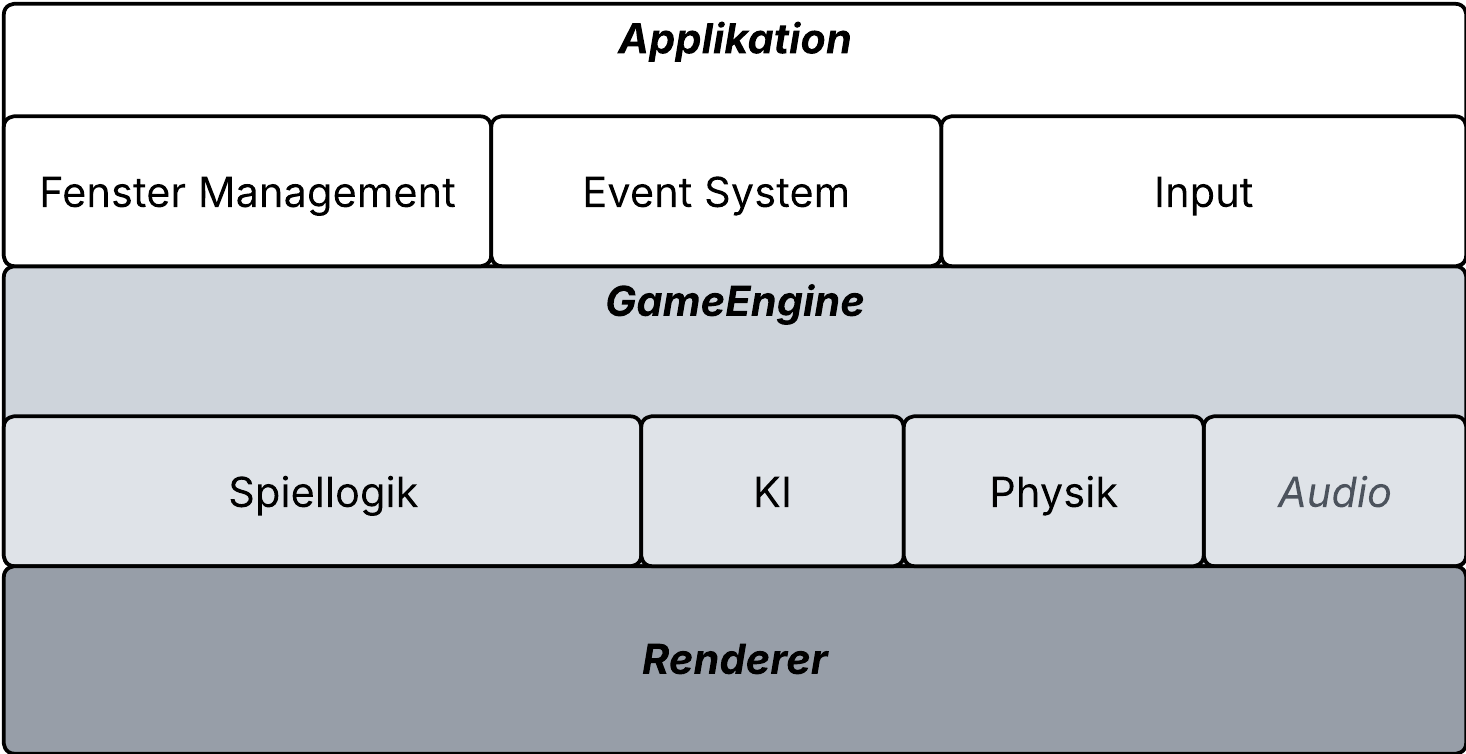
\includegraphics[width=1\columnwidth]{appendix/img/architecture}
    \caption{Vereinfachte Darstellung der Schichtenarchitektur des umzusetzenden Spiels. Das Audio-System ist hierbei berücksichtigt, auch wenn es bzgl. des Scopes keine Priorität hat.}
    \label{fig:architecture}
\end{figure}

\\


Die Physikengine soll auf die Anforderungen eines 2D-Shooters hin ausgerichtet sein (Bewegungsphysik basierend auf einfachen Vektoren in einer Ebene), die Kollisionsabfrage soll zuverlässig und performant funktionieren.


\subsection{Zielsetzung}

Diese Projektarbeit setzt den Fokus auf eine saubere Architektur sowie eine nachvollziehbare Umsetzung in der Programmiersprache C++$\ge$20.\\
Für die Darstellung des Spiels wird auf geometrische Primitive zurückgegriffen, so dass am Schluss ein Spiel entsteht das komplett auf Sprites verzichtet und die Darstellung aller benötigten Spielinformationen über Polygone und Linien realisiert (Fonts ausgenommen).

\noindent
Ein (messbarer) Schwerpunkt des Spiels ist eine stabile Framerate von $\ge$ 60 FPS bei einer Auflösung von $1920 \times 1080$.
Für die Entwicklung steht eine Grafikkarte vom Typ \textit{Nvidia GeForce RTX 5090} zur Verfügung, getestet werden kann außerdem auf einem Laptop mit einer \textit{Nvidia GTX 1070} Grafikkarte.
Die Lastparameter können also durchaus noch angepasst werden.\\
Die Herausforderung besteht hier in der anzuwendenden Technik bei der Darstellung von mehreren Hundert Gegnerobjekten auf dem Screen zur selben Zeit (\textit{Instancing}), Kollisionsabfrage mit dem Spieleschiff sowie den abgefeuerten Waffen und dem Gegnerverhalten bei entsprechender Steuerung des Spielerschiffes.\\
Ein nicht unwesentlicher Punkt bei der Umsetzung des Spiels ist der \textit{Game Feel}(\cite{Swi08})\footnote{
auch: \textit{Game Juice}
}: Das Spielererlebnis soll durch visuelles Trefferfeedback durch Partikeleffekte unterstützt werden.\\

\noindent
Die Gegner-KI basiert auf einem einfachen \textit{Spawn and Seek}-Verhalten mit einer zusätzlichen Drift-Komponente, die je nach Gegnertyp variiert. Für die Umsetzung sind 2-3 grundlegende Gegnertypen geplant:
\begin{itemize}
\itemsep0.5em
\item \textbf{Schneller Typ:} Geringe Widerstandsfähigkeit (wenig Schilde).
\item \textbf{Langsamer Typ:} Hohe Widerstandsfähigkeit (viele Schilde).
\item \textbf{Schwarm-Typ:} Mittlere Geschwindigkeit, keine Schilde, tritt in großer Anzahl als exklusive Gegnerwelle auf.
\end{itemize}

\noindent
Zur Steuerung des Spiels wird ein Gamecontroller wie der Xbox Elite Controller\footnote{
\url{https://www.xbox.com/de-DE/accessories/xbox-elite-controllers}
} bzw. der PS5 DualSense Wireless Controller\footnote{
\url{https://www.playstation.com/de-de/accessories/dualsense-wireless-controller/}
} vorausgesetzt.

\subsection{Vorgeschlagener Zeitplan}

\begin{itemize}
\itemsep0.5em
\item 20.10.2025: Bereitstellung der Applikationsschicht inkl. Implementierung des Event Systems, Input Managers sowie Anbindung an das Low Level API-Sub-Systems
\item 17.11.2025: Bereitstellung der Rendering Engine. Erster Entwurf des Spielfeldes samt Darstellung des Spielerschiffs.
\item 22.12.2025: Umsetzung der Physik und Spielereingabe zur Steuerung des Schiffs, Feuermechaniken
\item 19.01.2026: Implementierung der wichtigsten Spielregeln - und Mechaniken. Spielfähiger Prototyp.
\item 09.02.2026: Bereitstellung des umgesetzten Prototyps. Feinschliff.
\item 16.03.2026: Abgabe der Dokumentation und Vorstellung des Projekts.
\end{itemize}

\end{appendices}

%%%%%%%%%%%%%%%%%%%%%%%%%%%%%%%%%%
    \clearpage
    \sloppy
    \printbibliography
    \fussy


\end{document}
